\section{Using yield forecast disagreement and macro disagreement in the UKF}
In this section, we illustrate the results obtained when using yield forecasts instead of the estimated demand disagreement. The approach is described in the previous section.

The UKF yields a model-implied measure of demand disagreement. This can be compared to the estimated demand disagreement presented in Section~II. Table~\ref{table:DemandDisagreementComparison} summarizes the key statistics of the model-implied demand disagreement relative to the estimated series. We find that the model-implied measures, whether based on the extended filtering with macroeconomic disagreement, closely resemble the estimated demand disagreement.

Importantly, the correlation between the principal component–based macro disagreement observation equation and the estimated series is 75.2\%, indicating a high degree of alignment. This suggests that both methods are able to extract the relevant component of demand disagreement. However, since the extended UKF relies on ad hoc assumptions, we argue that the measure presented in Section~II is more suitable for our analysis.


\begin{table}[H]
    \centering
    \begin{tabular}{lccc}
        \toprule
        & \multicolumn{2}{c}{\textbf{Demand Disagreement}} \\
        \cmidrule(lr){2-4}
        & \textbf{Model Implied (PCA$_t$)} & \textbf{Model Implied (Regression)} & \textbf{Estimated} \\
        \midrule
        Mean        & 0.00465 & 0.00306 & 0.00383 \\
        Std.\ Dev.  & 0.00184 & 0.00261 & 0.00151 \\
        AC(1)       & 0.8323  & 0.956   & 0.70334 \\
        \midrule
        Correlation & 0.752   & 0.608   & -- \\
        \bottomrule
    \end{tabular}
    \vspace{0.5em}
    \caption{Summary statistics for estimated and model-implied demand disagreement. The left column shows values based on the first principal component ($PCA_t$) from macro disagreement; the middle column shows values from regressing yield disagreement onto macro disagreement and using the fitted values.}
    \label{table:DemandDisagreementComparison}
\end{table}

We also compare the model-implied state variables from the three different methods. Specifically, we extract $f_t$ and $l_t$ using the UKF approach from Section~V and the two alternatives introduced above. Table~\ref{tab:filtered_state_vars} presents the correlations and summary statistics of the filtered state variables across methods. The results show that the variables are highly correlated and share similar properties across approaches.


\begin{table}[H]
    \centering
    \caption{Comparison of Filtered State Variables Across Methods}
    \label{tab:filtered_state_vars}
    \vspace{0.5em}
    
    \textbf{Correlation of $f_t$} \\
    \begin{tabular}{lccc}
        \toprule
        & \textbf{Baseline} & \textbf{Macro} & \textbf{PCA} \\
        \midrule
        Baseline & 1.000 & 0.873 & 0.868 \\
        Macro    &       & 1.000 & 0.859 \\
        PCA      &       &       & 1.000 \\
        \bottomrule
    \end{tabular}

    \vspace{1em}
    
    \textbf{Correlation of $l_t$} \\
    \begin{tabular}{lccc}
        \toprule
        & \textbf{Baseline} & \textbf{Macro} & \textbf{PCA} \\
        \midrule
        Baseline & 1.000 & 0.853 & 0.831 \\
        Macro    &       & 1.000 & 0.908 \\
        PCA      &       &       & 1.000 \\
        \bottomrule
    \end{tabular}

    \vspace{1em}
    
    \textbf{Summary Statistics for $f_t$} \\
    \begin{tabular}{lccc}
        \toprule
        & \textbf{Mean} & \textbf{Std.\ Dev.} & \textbf{AC(1)} \\
        \midrule
        Baseline & 0.597 & 0.242 & 0.911 \\
        Macro    & 0.671 & 0.324 & 0.980 \\
        PCA      & 0.528 & 0.286 & 0.946 \\
        \bottomrule
    \end{tabular}

    \vspace{1em}
    
    \textbf{Summary Statistics for $l_t$} \\
    \begin{tabular}{lccc}
        \toprule
        & \textbf{Mean} & \textbf{Std.\ Dev.} & \textbf{AC(1)} \\
        \midrule
        Baseline & 0.975 & 0.475 & 0.988 \\
        Macro    & 1.428 & 1.079 & 0.994 \\
        PCA      & 0.623 & 0.427 & 0.982 \\
        \bottomrule
    \end{tabular}
\end{table}
Figure~\ref{fig:FilteredStates} plots the time series of $f_t$ and $l_t$ for the three filtering methods. As seen, all methods capture the same general trends and cycles. Notably, $l_t$ rises more sharply when using the regression-based macro disagreement compared to the PCA and baseline methods.

\begin{figure}[H]
    \centering
    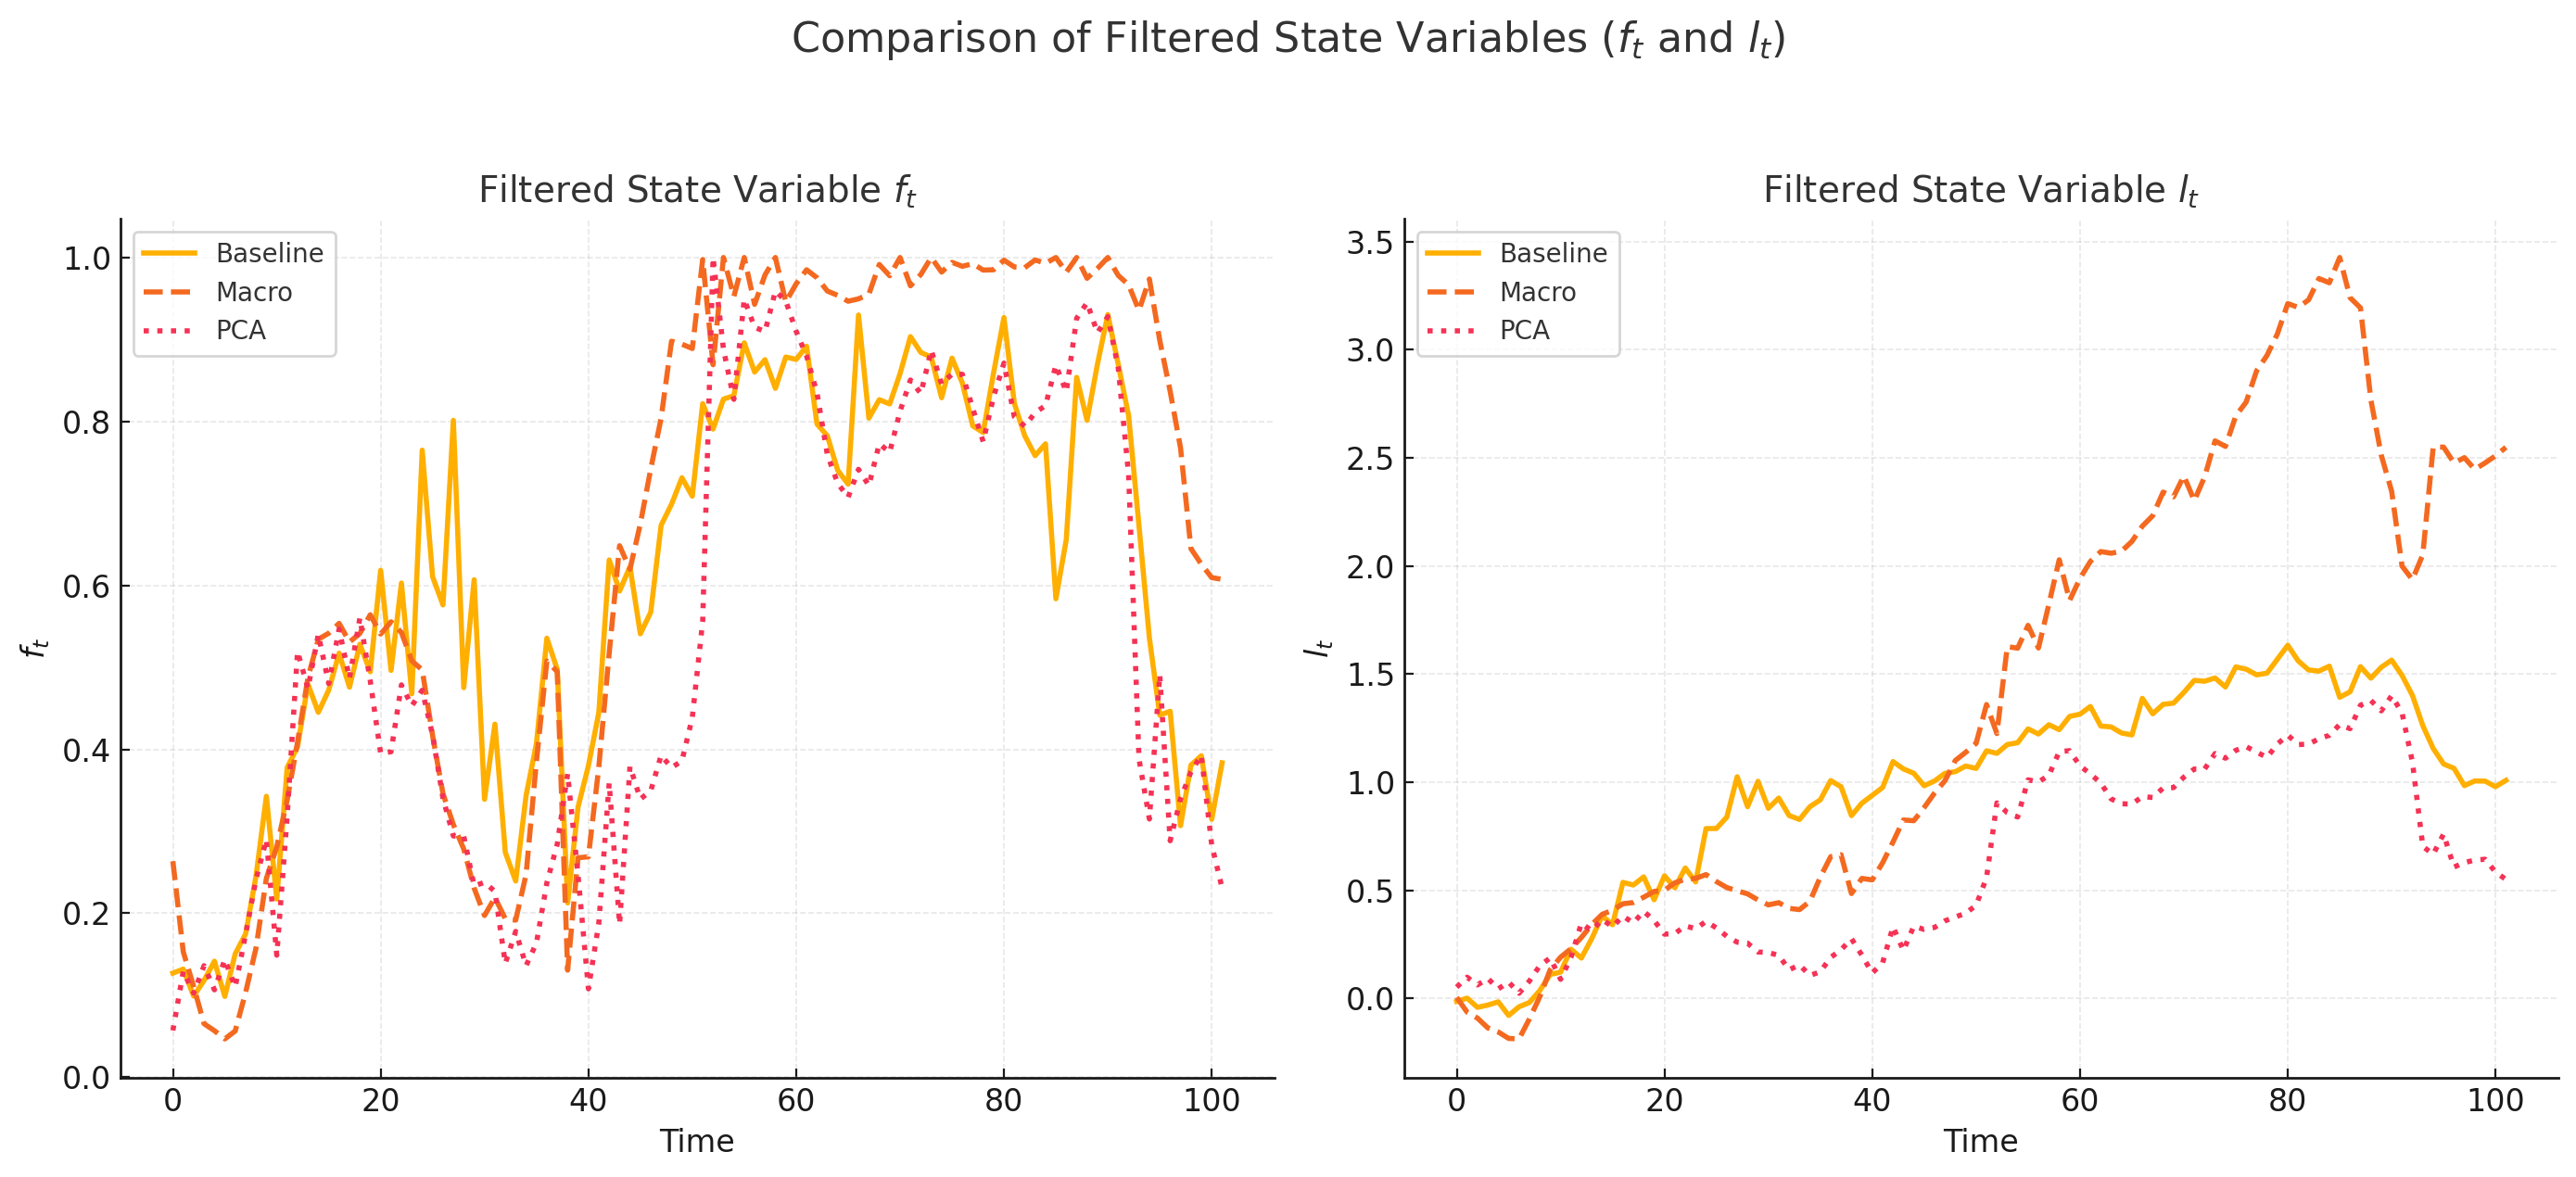
\includegraphics[width=\textwidth]{figures/Filter.png}
    \caption{Filtered state variables $f_t$ and $l_t$ across different specifications: the baseline model from Section~V, the regression-based model using macro disagreement, and the PCA-based model. The time series are closely aligned, indicating robustness of the filtering approach.}
    \label{fig:FilteredStates}
\end{figure}

Finally, we examine the behavior of other model-implied moments not explicitly used in the filtering process. Specifically, we regress the observed data on the model-implied time series for the 2-, 3-, 5-, 7-, and 10-year TIPS yields and their volatilities. We also include the slope of the yield curve, and regress realized excess returns on nominal bonds with 2-, 3-, and 5-year maturities.

This analysis mirrors the one in Section~V. Tables~\ref{table:AltUKFOOS} and~\ref{table:NewUKFOOS} present the results, which remain broadly consistent with the baseline model. It is worth noting that this constitutes a very stringent test of the model. We are using only two state variables, driven by a single shock, to back out implied time series for five yields, five volatilities, and three bond risk premia. Hence, overly strong results should not be expected.


\begin{landscape}
\begin{table}[H]
    \centering
    \begin{tabular}{lccccccccc}
        \toprule
        \multirow{2}{*}{\textbf{Maturity}} &
            \multicolumn{3}{c}{\textbf{Real Yields}} &
            \multicolumn{3}{c}{\textbf{Real Yield Volatilities}} &
            \multicolumn{3}{c}{\textbf{Nominal Bond Risk Premia}} \\
        \cmidrule(lr){2-4}\cmidrule(lr){5-7}\cmidrule(lr){8-10}
        & \textbf{Coeff.} & \textbf{Std.\ Dev.} & \textbf{R$^2$} 
        & \textbf{Coeff.} & \textbf{Std.\ Dev.} & \textbf{R$^2$} 
        & \textbf{Coeff.} & \textbf{Std.\ Dev.} & \textbf{R$^2$} \\
        \midrule
        2 years  & 0.544 & 0.076 & 0.553 & 0.063 & 0.057 & 0.011 & 0.964 & 0.509 & 0.091 \\
        3 years  & 0.535 & 0.069 & 0.604 & 0.073 & 0.046 & 0.028 & 1.201 & 0.623 & 0.087 \\
        5 years  & 0.525 & 0.061 & 0.642 & 0.070 & 0.031 & 0.061 & 1.250 & 0.653 & 0.080 \\
        7 years  & 0.519 & 0.057 & 0.650 & 0.060 & 0.029 & 0.059 & --    & --    & --    \\
        10 years & 0.520 & 0.054 & 0.654 & 0.046 & 0.028 & 0.046 & --    & --    & --    \\
        Slope    & 0.622 & 0.288 & 0.091 & --    & --    & --    & --    & --    & --    \\
        \bottomrule
    \end{tabular}
    \vspace{0.5em}
    \caption{Regression Results: Yields, Yield Volatilities, and Bond Risk Premia}
    \label{table:AltUKFOOS}
    \begin{minipage}{0.95\textwidth}
        \footnotesize
        Coefficients come from $y^{\text{Data}}_t = a + b\,y^{\text{Model}}_t + u_t$ for each series and maturity.
        Dashes denote unavailable observations. The measurement equations is based on the yield disagreement, the two year TIPS and $PCA_t$. Despite deviations of the slope estimates from one, the positive signs and
        $R^2$ values confirm that the model captures salient features of the data.
    \end{minipage}
\end{table}
\end{landscape}

\begin{landscape}
\begin{table}[H]
    \centering
    \begin{tabular}{lccccccccc}
        \toprule
        \multirow{2}{*}{\textbf{Maturity}} &
            \multicolumn{3}{c}{\textbf{Real Yields}} &
            \multicolumn{3}{c}{\textbf{Real Yield Volatilities}} &
            \multicolumn{3}{c}{\textbf{Nominal Bond Risk Premia}} \\
        \cmidrule(lr){2-4}\cmidrule(lr){5-7}\cmidrule(lr){8-10}
        & \textbf{Coeff.} & \textbf{Std.\ Dev.} & \textbf{R$^2$} 
        & \textbf{Coeff.} & \textbf{Std.\ Dev.} & \textbf{R$^2$} 
        & \textbf{Coeff.} & \textbf{Std.\ Dev.} & \textbf{R$^2$} \\
        \midrule
        2 years  & 0.753 & 0.060 & 0.716 & 0.070 & 0.074 & 0.020 & 1.231 & 0.728 & 0.079 \\
        3 years  & 0.710 & 0.055 & 0.730 & 0.082 & 0.060 & 0.055 & 1.180 & 0.882 & 0.046 \\
        5 years  & 0.653 & 0.056 & 0.701 & 0.068 & 0.038 & 0.086 & 0.646 & 0.914 & 0.012 \\
        7 years  & 0.614 & 0.057 & 0.660 & 0.051 & 0.031 & 0.062 & --    & --    & --    \\
        10 years & 0.581 & 0.059 & 0.611 & 0.027 & 0.025 & 0.022 & --    & --    & --    \\
        Slope    & 1.978 & 0.360 & 0.457 & --    & --    & --    & --    & --    & --    \\
        \bottomrule
    \end{tabular}
    \vspace{0.5em}
    \caption{Regression Results: Yields, Yield Volatilities, and Bond Risk Premia}
    \label{table:NewUKFOOS}
    \begin{minipage}{0.95\textwidth}
        \footnotesize
        The table reports coefficients from the regression 
        $y^{\text{Data}}_t = a + b\,y^{\text{Model}}_t + u_t$
        for different maturities. The measurement equations is based on the yield disagreement, the two year TIPS and the prediction from regressing the yield disagreement onto macro disagreement. Although the estimated slopes differ from one, their magnitudes,
        signs, and associated $R^2$ values indicate the model still captures key features of the data.
        Dashes denote maturities for which a particular series is not available.
    \end{minipage}
\end{table}
\end{landscape}

